\documentclass[12pt, a4paper]{article}
\usepackage{geometry}
\renewcommand{\baselinestretch}{1.15}
\usepackage[backend = biber, citestyle = authoryear, url = false]{biblatex}
\usepackage{hyperref}
\usepackage{pdflscape}
\usepackage{graphicx}
\addbibresource{sop.bib}
\title{Is small beautiful? Do small districts lead to better outcomes?}
\author{Jothsna Rajan \\
	\small{Indian Institute of Management, Bangalore, India}}
\geometry{a4paper, top=25mm}
\graphicspath{ {Images/} }
\usepackage{Sweave}
\begin{document}
\Sconcordance{concordance:seminar.tex:seminar.Rnw:%
1 13 1 1 0 131 1 1 15 1 1 1 4 44 0 1 3 1 16 40 0 1 23 39 0 1 2 1 13 40 %
0 1 23 39 0 1 2 1 11 15 1 1 16 40 0 1 21 39 0 1 3 1 16 40 0 1 22 39 0 1 %
2 1 15 34 0 1 7 46 0 1 7 46 0 1 7 46 0 1 2 3 5 2 1}

	\maketitle
\begin{abstract}
	What is the optimal population level for local public service delivery? Recent debates on the topic attribute considerable virtues to small jurisdictions. But does bifurcating larger districts into smaller ones pay off? I examine this question in the context of public education using data from a district bifurcation process in Karnataka, India. The performance of sub-districts which were allocated to newly created smaller districts is compared with sub-districts that remained in larger districts using a difference in difference estimation model. Education performance outcomes and service delivery are measured in test scores, as well as inputs to schooling such as the number of schools, funding for schools, number of academic inspections conducted per year, etc. The results seem to suggest that there is no significant improvement in education outcomes or service delivery as a result of the bifurcation. 
\end{abstract}
\paragraph{} Is there an optimal size for local government systems? Aristotle in his treatise `Politics' argued that political entities needed to balance the twin considerations of economic viability and effective citizenship \parencite{aristotle_politics_1984}. In modern democracies, debates on the topic are framed in a similar language with two sets of normative criteria. The first one is \textit{output legitimacy}. The function of local governments is to provide a set of public goods and services to its citizens and promote public welfare. A government that fulfils this duty better has higher output legitimacy. The other normative concern is `citizen effectiveness' or the capability and willingness of citizens to control the decisions made on their behalf \parencite{dahl_size_1973}. Enhancing citizen effectiveness raises the \textit{input legitimacy} of the system. Both output and input legitimacy are prerequisites to democratic legitimacy \parencite{scharpf_governing_1999}. The fundamental assumption in these debates is that changing the size of political units is likely to affect the democratic quality (input legitimacy) and functional effectiveness (output legitimacy) of governments. 
	
\paragraph{} Recent debates on the topic attribute considerable virtues to small jurisdictions. In democratic societies, the economic and political arguments tend to converge. Small jurisdictions are believed to enhance political participation, make politics less abstract, politicians more responsive, and facilitate exit-based empowerment of citizens \parencite{hansen_size_2014}. Decentralisation will also increase economic efficiency as the local governments have an information advantage and can respond better to variance in preferences at the local level \parencite{oates_fiscal_1972}, and population mobility will lead to competition between local authorities and better provision of public goods. Decentralised service delivery especially when citizens directly elect the local governments is expected to provide better coverage, quality and efficiency \parencite{smoke2015rethinking}. Competing local governments may experiment with various ways to provide public goods and lead to innovations that can be applied elsewhere. At the same time there is a counter argument in favour of larger jurisdiction sizes because it allows for economies of scale in the providing public goods \parencite{hirsch_expenditure_1959}. These considerations suggest that public goods that are (1) sensitive to local preferences and (2) do not have large spillover (3) nor scale effects: infrastructure, public education, etc. are better provided under decentralisation (\cite{tiebout_economies_1960}, \cite{oates_fiscal_1972}). 
	
\paragraph{} In a bid to arrive at the optimal population size in a local government unit, many national governments have reorganised their sub-national boundaries. Europe has seen local government consolidation via municipal amalgamations while transitional economies have seen increasing decentralisation at the local government level. Since the 1950s, India has seen frequent administrative bifurcations at the local government level (district level). The number of districts in the country has increased from 356 in the 1971 census period to 640 in the 2011 census (Table. \ref{Fig2}) This is a trend that is continuing to the present day. West Bengal has created five new districts since 2015. The rationale for creating new districts was stated to be - ``...for \textit{better administrative control,} and so that \textit{public service can be delivered at the door steps} of the people staying at remote areas'' (emphasis added) \parencite{Mamata}. Similarly, Telangana state is contemplating the creation of 14 - 15 new districts \parencite{Telengana} and Haryana state is considering three more districts \parencite{Haryana}. In all these cases, the stated rationale for district bifurcation is decentralisation of administration and better public service. And India is not alone in the implementation of administrative bifurcations at the local government level. Brazil, in the period from 1990 to 2000, increased the number of municipalities from 4,491 to 5,560 \parencite{tomio2005creation}. Russia adopted Local Government Reform in 2003 and since then has doubled the number of municipalities \parencite{turgel2008new}\nocite{avellaneda_is_2015}. But does creating new districts enhance public service outcomes?
	
	\begin{table}[h!]
		\centering
		\caption{New Districts created in India across Census Periods}
		\label{Fig1}
		\begin{tabular}{c|cccc} 
			\hline
			States/UTs & 1971-81 & 1981-91 & 1991-2001 & 2001-11 \\
			\hline 
			Andaman and Nicobar Islands & 1 & 0 & 0 & 1  \\ 
			Andhra Pradesh & 2 & 0 & 0 & 0  \\ 
			Arunachal Pradesh & 4 & 2 & 2 & 3  \\ 
			Assam & 0 & 13 & 0 & 4  \\ 
			Bihar & 14 & 11 & 8 & 1  \\ 
			Chhattisgarh & 0 & 0 & 9 & 2  \\ 
			Daman and Diu & 0 & 2 & 0 & 0  \\ 
			Delhi & 0 & 0 & 8 & 0  \\ 
			Goa & 0 & -1 & 0 & 0  \\ 
			Gujarat & 0 & 0 & 6 & 1  \\ 
			Haryana & 5 & 4 & 3 & 2  \\ 
			Himachal Pradesh & 2 & 0 & 0 & 0  \\ 
			Jammu and Kashmir & 4 & 0 & 0 & 8  \\ 
			Jharkhand & 0 & 0 & 5 & 6  \\ 
			Karnataka & 0 & 1 & 7 & 3  \\ 
			Kerala & 2 & 2 & 0 & 0  \\ 
			Madhya Pradesh & 2 & 0 & 7 & 5  \\ 
			Maharashtra & 0 & 4 & 5 & 0  \\ 
			Manipur & 1 & 2 & 1 & 0  \\ 
			Meghalaya & 3 & 0 & 2 & 0  \\ 
			Mizoram & 3 & 0 & 5 & 0  \\ 
			Nagaland & 4 & 0 & 1 & 3  \\ 
			Odisha & 0 & 0 & 17 & 0  \\ 
			Punjab & 1 & 0 & 5 & 3  \\ 
			Rajasthan & 0 & 1 & 5 & 1  \\ 
			Tamil Nadu & 2 & 5 & 9 & 2  \\ 
			Tripura & 0 & 0 & 1 & 0  \\ 
			Uttar Pradesh & 2 & 7 & 16 & 1  \\ 
			Uttarakhand & 0 & 0 & 4 & 0  \\ 
			West Bengal & 0 & 1 & 1 & 1  \\ 
			\hline
			Overall & 52 & 54 & 127 & 47  \\ 
			\hline
		\end{tabular}
	\end{table} 
	
\paragraph{}This paper explores the effect of bifurcation of districts on public service outcomes - specifically, the quality of public education. I present the theory behind reorganisation and the available evidence on its effectiveness, and discuss the methodological challenges in the empirical examination of size effects. I test my propositions using data collected on public education in the districts of Karnataka in India over a nine year period from 2005 to 2013. Karnataka created three new districts by bifurcating three existing ones during the period. Remaining districts were left untouched. A new district is created by reallocating some of the taluks (sub-districts) within an existing district to a new one. This allows use of a difference in difference model to test for the effect of the policy on education outcomes. The reform was driven by the state government, following public demand for creation of new districts and had taken place at different times. But the rationale for the public demand was based on cultural factors rather than public education concerns. My findings suggest that for the most part there is no significant impact of the district reorganisation on the public education outcomes or service delivery in the years after the split.
	
\section*{Theory}
\paragraph{} The fundamental argument for decentralised governance comes from the perspective that there is heterogeneity in demand for public services. The variance in preferences can be better understood and catered to by a government that is closer to the citizens, thus raising well-being throughout society. Tiebout, in his 1956 paper, talks about citizens \textit{voting with their feet} or \textit{exiting}. He conceptualises a fully mobile citizen that can move to a jurisdiction that matches her preferences for tax rates and public service levels, thus revealing her preferences \parencite{tiebout_economies_1960}. Thus with small jurisdictions this information can be used by local governments to tailor their activities and raise welfare. But how much decentralisation should we demand? Oates' Decentralization Theorem formalizes it as \textit{``...in the absence of cost-savings from the centralized provision of a [local public] good and of inter jurisdictional externalities, the level of welfare will always be at least as high (and typically higher) if Pareto-efficient levels of consumption are provided in each jurisdiction than if any single, uniform level of consumption is maintained across all jurisdictions''}(\cite{oates_fiscal_1972}, pg 54). \nocite{oates1999essay}
	
\paragraph{} In other words, a public good that does not have large economies of scale or inter-jurisdictional externalities may be better provided under decentralisation. Public education is not seen as imposing strong externalities on neighbouring regions, nor does it have large scale effects. Therefore, under the classic explanation, a smaller district should be able to provide better service. At the same time, practical considerations remain. We might need to build administrative capacity when a larger district is split into two or more before any benefits can be reaped. Also, if the districts are too small in the first place, there might be some benefit in consolidating two or more districts and managing them together.  
	
\paragraph{Jurisdiction Size} Administrative bifurcations lead to lowering of the jurisdiction size and are often pursued in hopes that smaller population sizes will lead to administrative convenience and better allocative efficiency. Smaller populations may reduce agency costs especially if the local administrators are directly elected and information costs because of the proximity of the decision-making-centre to the citizens. It may also lead to lower costs in planning and monitoring activities than in a larger jurisdiction. At the same time, it can lead to higher costs by administrative duplication. Creation of a new district entails additional administrative costs as the new districts often need to create the administrative infrastructure. Some of these effects are likely to materialise over a longer period and would require a long research period. On the other hand, a larger jurisdiction size will allow you to spread fixed costs of a greater population. \nocite{allers2016effects} \nocite{lassen_jurisdiction_2011} The optimal jurisdiction size at which public service delivery begins to improve or decline might also be a function of the specific public good or service. It also needs to be stated that the effects of size on public service delivery depends on the size of production units as well, not just administrative units. For example, in the case of public education, a smaller district may recognise the need for higher educational spending and raise the number of schools in the region accordingly, but the educational outcomes or test scores would depend on the size and characteristics of the schools as well. 
	
\paragraph{Service Levels} Decentralised governance is expected to make government more responsive to the citizens. If there is heterogeneity in preferences, it may be reflected in levels of public service delivered. Smaller administrative units allow the tailoring of public services to the preferences of smaller and more homogenous groups thus achieving greater allocative efficiency of public budgets. %Conditional on the variation in preferences a district after bifurcation may exhibit divergence in service levels. If preferences are more homogeneous, then there will be less need to deviate from previous service levels. 
There is some evidence from the decentralisation reforms in Bolivia and Columbia to suggest that decentralisation has enhanced the local allocative efficiency of public funds. Notably, it has resulted in shifting resources towards education in regions where education performance has historically been worse. But data limitations prevent the authors from testing whether the improvement extends to education outcomes, such as literacy and test scores \parencite{faguet2008decentralization}. Also, there is evidence from California state, to suggest that students in smaller districts perform better than those in larger districts in standardised tests after controlling for a variety of other factors \parencite{driscoll2003school}.

\paragraph{} The critics of decentralisation argue that its effectiveness is often greatly hampered by the particular context of its implementation. Vito Tanzi offers an argument for corruption to be higher at local levels than at central government levels, because of closer interaction at the local level between the bureaucrats and citizens that can enable nepotism and personal favours \parencite{tanzi1996macroeconomic}. Also, local bureaucracies may be poorly staffed and ill-equipped to handle the responsibilities associated with the decentralised provision of public goods \parencite{prud1995dangers}. The precise nature of decentralisation, such as the financial autonomy of the local government may also pay a role in determining whether the benefits can be reaped. 
	
\paragraph{}  The effect of any form of administrative reorganization - bifurcation or consolidation (or a combination of both) - depends on the particular context and capabilities of the local administrative body. Holzer et al in 2009 provides a review of the empirical literature on this question. Their review suggests that the evidence on the effect of size on local government performance is inconclusive - there is very little correlation between size and efficiency for population sizes between 25,000 and 250,000 - anything above that or below is less efficient \parencite{holzer2009literature}. These factors caution against the implementation of decentralisation as a panacea for administrative ills. It also means that any instance of decentralisation can be explored further to understand the context of success or failure. But administrative bifurcation at the local government level is a step that is frequently taken - despite the lack of strong evidence in its favour. 
	
\section*{Endogeneity and Empirical Strategy}
\paragraph{} Spatial and temporal variation in public policy affords the conditions suitable for identifying the impact of the policy on outcomes. But the size and boundary of the administrative unit is an active response to a problem and is endogenous - it can be included in the left \textit{or} right side of the estimation equation. In this paper, I use a difference in difference estimation comparing the changes in performance of districts that were divided to a control group of districts that were not divided in order to estimate the effect of the bifurcation of the administrative district on the public spending and quality of educational service delivered. The DID estimation strategy requires that the error term be uncorrelated with the bifurcation status. This is unlikely as the districts that were split may be different from those that were not. The demand for creation a new district usually arises from within the district and the political traction gained by the idea has a role to play in the eventual decision made by the state. If the source of variation in policy action arises from within the characteristics of the intended beneficiaries of the policy, then we have a policy endogeneity. 
	
\paragraph{} To control for the policy endogeneity or self-selection into treatment, it is possible to use an instrumental variable approach. A good instrument would be a variable that influences the choice of a district to be bifurcated and is otherwise independent of the quality of public service delivery and outcomes in the region. As the stated rationale for creating new districts in India is administrative convenience, population at the district level at the 2001 census is likely to make a good instrument. Larger districts are more likely to be perceived as unwieldy and seen as candidates for bifurcation. At the 2001 census, Karnataka state had 27 districts - each with an average population of over 660,000 (If we exclude the urban district of Bangalore, the average drops to around 470,000). Between 2007 and 2010 three new districts were carved out from three existing ones. Two new districts (Chikballapura and Ramanagara) were created from two existing ones (Kolar and Bangalore Rural respectively) in 2007, and a third new district (Yadgir) was created from an existing one (Gulbarga) in 2010 taking the total in the state up to 30. The instrumental variable approach though plausible, is not employed in this study as the sample size is too small to support it. 

\paragraph{}The approach that is considered here is to include the variables that may influence selection in the model. This is not perfect as all potential explanatory variables that may bias the choice cannot be captured. I also use two different control groups against which the bifurcated districts are compared. First group consists of all the other sub-districts in the state - except for those from Bangalore Urban district, which is a clear outlier. The second control group is chosen by using propensity scores to match sub-districts that have similar observable characteristics. 
\subsection*{Data}
The sub-district level data on public education is provided by District Information System for Education (DISE). Data is available at the school level on infrastructure and resources and is aggregated to the sub-district level for the analysis here. Student performance data is taken from the annual Secondary School Leaving Certificate (SSLC) examination. All students in the state at the close of their secondary education appear for the SSLC exam, which forms a gateway to any future educational or vocational plans. The exam is conducted statewide by the Karnataka Secondary Education Examination Board (KSEEB). I obtain data on exam results at the student level for control and treatment taluks for the exams conducted in April 2006 to April 2014. The unit of analysis is the subdistrict and each subdistrict is given a treatment (bifurcation) status of 0 or 1 based on whether in 2005 it belonged to a district that was subsequently bifurcated. 
\paragraph{} I have used demographic data from the closest census (Census 2001) to identify control groups using propensity scores from the baseline (Academic Year 2005-06). The variables considered for propensity score matching are school performance, number of schools per 1000 population, average number of female teachers in the schools across the sub-district, proportion of schools in the subdistrict with electricity, proportion of government funded schools, average number of graduate teachers, number of households, population less than 6 years of age, literate population and scheduled castes and scheduled tribes population. 

\begin{figure}[h!]
	\centering
	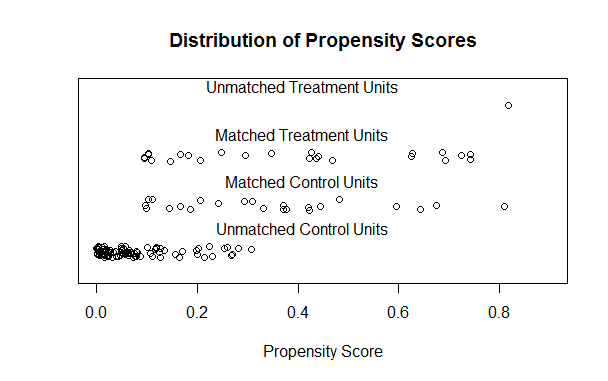
\includegraphics[scale = 0.85]{Jitter}
	\caption{Propensity Score Matching: Jitter Plot}
	\label{Fig1}
\end{figure}

\begin{figure}[h!]
	\centering
	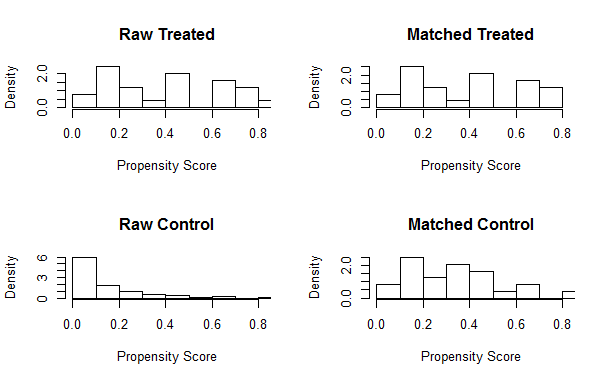
\includegraphics[scale = 0.85]{PSMatch}
	\caption{Propensity Score Matching: Histogram}
	\label{Fig2}
\end{figure}


The default specification is of the form,

\[ Y_{it} = \beta_0 + \beta_1 Split_{i} + \beta_2 PostSplit_t + \beta_3 Split_i PostSplit_t + \beta_j X_{ijt} + \epsilon_{it} \]

Academic Year 2013-14 is taken as the post treatment period (PostSplit = 1). The bifurcation itself happened in two instances - one is 2007 and the other in 2010. But in most instances, the bifurcation is notified by the government before the administrative machinery is setup. In effect, the district is bifurcated on paper, but the administrative responsibilities rest on the same shoulders as before in the immediate aftermath. Overtime the administrative machinery of the new district is set up and positions filled. This process may take two to three years. The academic year ending in 2014 is chosen as it gives sufficient time for the new districts created in 2007 and 2010 to find their feet.

\begin{figure}[h!]
	\centering
	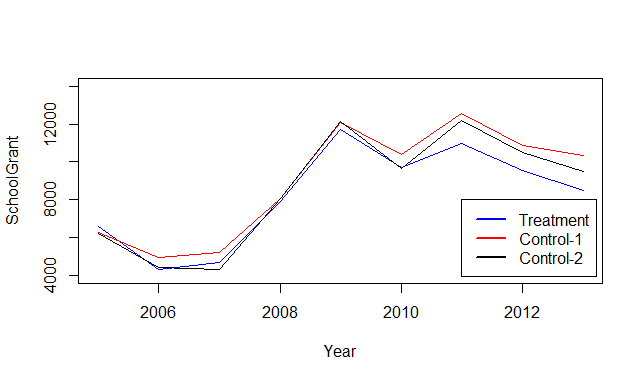
\includegraphics[scale = 0.85]{SchoolGrant}
	\caption{School Grant for Treatment and Control Groups}
	\label{Fig3}
\end{figure}

\begin{figure}[h!]
	\centering
	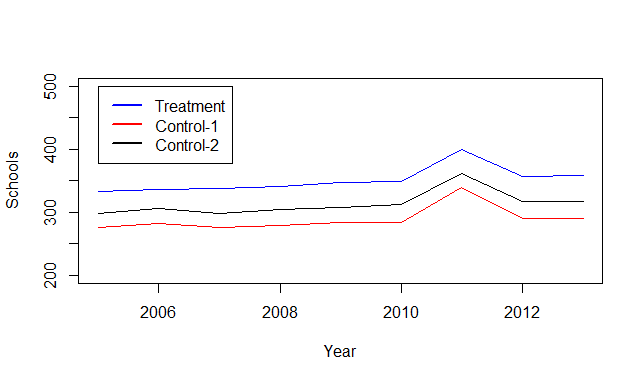
\includegraphics[scale = 0.85]{Schools}
	\caption{No of Schools for Treatment and Control Groups}
	\label{Fig4}
\end{figure}

\paragraph{} The outcome variables that are evaluated can be considered in three groups. First is the \textit{Investment variables}. As the name suggests these are variables that indicate the local governments investments in schools. This includes proportion of public schools, total number of school and grants allocated to schools to procure materials and to perform minor infrastructural improvements and repairs. These are small grants - the average figure is less than 10,000 per year, though there is significant variation across schools. Two indicators for investment in schools - number of schools and the amount of school grant are plotted for the bifurcated districts and the two control groups in Fig. \ref{Fig3} and \ref{Fig4}. The treatment and control groups follow closely matching trends in the number of schools and diverge slightly in the amount of school grants - with the treatment groups receiving less grants in total than either of the control groups. The second group is the group of \textit{Resources variables}. They include physical infrastructure indicators such as classroom, electricity and library, quality of teachers, and quality of oversight such as number of academic inspections. The third kind of variable is the student \textit{Performance Variable} and is measured as a test scores in the SSLC exam. The results presented in Table. \ref{Table2} are with the control group matched using propensity scores (Control Group 2). Remaining tables are included in the appendix.
\nocite{hinnerich2009merging} \nocite{jordahl2010merged} \nocite{reingewertz2012municipal} \nocite{blesse2013municipal}. 

\paragraph{} The results of the estimation model shows insignificant effects of the bifurcation on most service delivery and performance outcomes. The districts that underwent decentralization on the whole seem to allocate less grants to schools than the ones that were not bifurcated. On the whole the districts that underwent bifurcation do not seem different from those that did not - except for a decline in school grants. Does that remain true within the bifurcated districts as well? In each bifurcated district, there are some taluks which remain with the older district with an already established administrative machinery - and some which were spun off into the new district and had to set up administration anew. Table \ref{Table3} examines whether the `new' districts are different from the `old' district within treatment. The p values from a t test are also included in the table and we can see that except for the average number of female teachers per school, all `new' districts are indistinguishable from the `old' in all characteristics. 

\begin{landscape}
	% Table created by stargazer v.5.2 by Marek Hlavac, Harvard University. E-mail: hlavac at fas.harvard.edu
	% Date and time: Thu, Jul 14, 2016 - 12:56:36 PM
	\begin{table}[!htbp] \centering 
		\caption{Basic Regression Results: With Control Group 2} 
		\label{Table2} 
		\scalebox{0.9}{
		\begin{tabular}{@{\extracolsep{5pt}}lcccccccc} 
			\\[-1.8ex]\hline 
			\hline \\[-1.8ex] 
			& \multicolumn{8}{c}{\textit{Dependent variable:}} \\ 
			\cline{2-9} 
			\\[-1.8ex] & ln(Grants) & \# of Schools & Public & Classrooms & Toilet-Girls & Electricity & Library & Test Scores \\ 
			\\[-1.8ex] & (1) & (2) & (3) & (4) & (5) & (6) & (7) & (8)\\ 
			\hline \\[-1.8ex] 
			Split & 0.3 & 0.1$^{*}$ & 0.001 & $-$0.5$^{***}$ & $-$0.001 & $-$0.04 & 0.04 & 0.2 \\ 
			& (0.2) & (0.1) & (0.02) & (0.2) & (0.001) & (0.04) & (0.1) & (7.8) \\ 
			& & & & & & & & \\ 
			Post & 0.9$^{***}$ & 0.2$^{***}$ & $-$0.1$^{***}$ & 0.2 & $-$0.01$^{***}$ & 0.3$^{***}$ & 0.1 & 10.0 \\ 
			& (0.2) & (0.1) & (0.02) & (0.2) & (0.002) & (0.1) & (0.1) & (19.0) \\ 
			& & & & & & & & \\ 
			Split:Post & $-$0.5$^{**}$ & $-$0.03 & $-$0.02 & 0.1 & 0.003$^{*}$ & 0.1 & 0.2 & 13.0 \\ 
			& (0.2) & (0.1) & (0.02) & (0.2) & (0.002) & (0.05) & (0.1) & (10.0) \\ 
			& & & & & & & & \\ 
			Demographic Variables & YES & YES & YES & YES & YES & YES & YES & YES \\
			Investment Variables & NO & NO & NO & YES & YES & YES & YES & YES \\
			Resource Variables  & NO & NO & NO  & NO & NO & NO & NO & YES \\
			\hline \\[-1.8ex] 
			Observations & 95 & 95 & 95 & 95 & 95 & 95 & 95 & 95 \\ 
			R$^{2}$ & 0.3 & 0.4 & 0.4 & 0.8 & 0.4 & 0.8 & 0.3 & 0.4 \\ 
			Adjusted R$^{2}$ & 0.2 & 0.4 & 0.3 & 0.8 & 0.3 & 0.8 & 0.2 & 0.4 \\ 
			Residual Std. Error & 0.6 & 0.2 & 0.1 & 0.5 & 0.005 & 0.1 & 0.3 & 24.0 \\ 
			F Statistic & 5.3$^{***}$ & 9.7$^{***}$ & 9.4$^{***}$ & 40.0$^{***}$ & 5.6$^{***}$ & 35.0$^{***}$ & 4.1$^{***}$ & 6.6$^{***}$ \\ 
			\hline 
			\hline \\[-1.8ex] 
			\textit{Note:}  & \multicolumn{8}{r}{$^{*}$p$<$0.1; $^{**}$p$<$0.05; $^{***}$p$<$0.01} \\ 
		\end{tabular} }
	\end{table} \end{landscape}

\begin{table}[!htbp] \centering 
	\caption{Summary Statistics in 2013 - Within Treatment Group} 
	\label{Table3} 
	\begin{tabular}{@{\extracolsep{5pt}} ccccc} 
		\\[-1.8ex]\hline 
		\hline \\[-1.8ex] 
		& Variables & Old & New & p.value \\ 
		\hline \\[-1.8ex] 
		1 & Total Marks & $344.0$ & $333.0$ & 0.33 \\ 
		2 & Rural/Urban (rural = 1) & $0.9$ & $0.9$ & 0.56 \\ 
		3 & Working Days & $0.7$ & $1.1$ & 0.57 \\ 
		4 & Academic Inspection & $1.3$ & $1.6$ & 0.67 \\ 
		5 & School Dev Grant - R & $7,260.0$ & $7,574.0$ & 0.6 \\ 
		6 & School Dev Grant - E & $6,542.0$ & $6,442.0$ & 0.76 \\ 
		7 & TLM Grant - R & $1,098.0$ & $1,456.0$ & 0.19 \\ 
		8 & TLM Grant - E & $1,017.0$ & $1,352.0$ & 0.18 \\ 
		9 & Classrooms & $4.9$ & $4.5$ & 0.2 \\ 
		10 & Electricity (Yes = 1) & $1.0$ & $1.0$ & 0.62 \\ 
		11 & Library  (Yes = 1) & $1.0$ & $1.2$ & 0.36 \\ 
		12 & PlayGround  (Yes = 1) & $0.6$ & $0.5$ & 0.57 \\ 
		13 & Male teachers & $2.1$ & $2.1$ & 0.94 \\ 
		14 & Female teachers & $2.4$ & $1.8$ & 0 \\ 
		15 & Grad teachers & $1.0$ & $0.7$ & 0.21 \\ 
		16 & ProfQ teachers & $4.4$ & $3.7$ & 0.03 \\ 
		17 & Days\_non teaching activity & $0.5$ & $0.1$ & 0.2 \\ 
		18 & Public Schools (\%) & $0.8$ & $0.9$ & 0.18 \\ 
		19 & Households & $45,379.0$ & $48,264.0$ & 0.66 \\ 
		20 & Total Population & $222,491.0$ & $236,014.0$ & 0.7 \\ 
		21 & Population 0 - 6 & $27,863.0$ & $30,597.0$ & 0.69 \\ 
		22 & Literates & $129,369.0$ & $119,382.0$ & 0.53 \\ 
		23 & Total W Population & $108,226$ & $121,141$ & 0.44 \\ 
		24 & SC/ST Population & $73,461.0$ & $84,702$ & 0.45 \\ 
		25 & No of Schools in Taluk & $333.0$ & $337.0$ & 0.93 \\ 
		26 & Schools per 1000 people & $1.5$ & $1.6$ & 0.77 \\ 
		27 & New/Old Dist (New = 1) & $0$ & $1$ & - \\ 
		28 & \# of Observations & $14$ & $9$ & - \\ 
		\hline \\[-1.8ex] 
		\multicolumn{5}{l}{Population figure used to calculate `Schools per 1000 people' is from 2001} \\ 
	\end{tabular} 
\end{table}

\section*{Conclusion}
\paragraph{} This paper explores the effect of district reorganization on the eventual public education delivery and outcomes. The findings suggest that there is 

\paragraph{} The findings from the study suggest no significant changes in the education outcomes of the sub-districts following a bifurcation. It is acknowledged here that government functions are many and varied and the effect of population size on one of those functions might not be the same as that on others. As such, this study cannot claim to comment on local government size without due consideration to other functions and services performed by local governments. Future iterations of this study would attempt to mitigate this issue to some extent by broadening the scope of services considered into public health and sanitation at a pan India setting.
\printbibliography
\pagebreak
\section*{Appendix}
\begin{table}[h!]
		\centering
		\caption{No\# of Districts in India - Statewise}
		\label{Fig2}
		\scalebox{0.9}{
		\begin{tabular}{c|ccccc} 
			\hline
			States/UTs & 1971 & 1981 & 1991 & 2001 & 2011 \\
			\hline 
			Andaman \& Nicobar Islands & 1 & 2 & 2 & 2 & 3 \\ 
			Andhra Pradesh & 21 & 23 & 23 & 23 & 23 \\ 
			Arunachal Pradesh & 5 & 9 & 11 & 13 & 16 \\ 
			Assam & 10 & 10 & 23 & 23 & 27 \\ 
			Bihar & 17 & 31 & 42 & 37 & 38 \\ 
			Chandigarh & 1 & 1 & 1 & 1 & 1 \\ 
			Chhattisgarh &  &  &  & 16 & 18 \\ 
			Dadra \& Nagar Haveli & 1 & 1 & 1 & 1 & 1 \\ 
			Daman \& Diu &  &  & 2 & 2 & 2 \\ 
			Delhi & 1 & 1 & 1 & 9 & 9 \\ 
			Goa & 3 & 3 & 2 & 2 & 2 \\ 
			Gujarat & 19 & 19 & 19 & 25 & 26 \\ 
			Haryana & 7 & 12 & 16 & 19 & 21 \\ 
			Himachal Pradesh & 10 & 12 & 12 & 12 & 12 \\ 
			Jammu \& Kashmir & 10 & 14 & 14 & 14 & 22 \\ 
			Jharkhand &  &  &  & 18 & 24 \\ 
			Karnataka & 19 & 19 & 20 & 27 & 30 \\ 
			Kerala & 10 & 12 & 14 & 14 & 14 \\ 
			Lakshadweep & 1 & 1 & 1 & 1 & 1 \\ 
			Madhya Pradesh & 43 & 45 & 45 & 45 & 50 \\ 
			Maharashtra & 26 & 26 & 30 & 35 & 35 \\ 
			Manipur & 5 & 6 & 8 & 9 & 9 \\ 
			Meghalaya & 2 & 5 & 5 & 7 & 7 \\ 
			Mizoram &  & 3 & 3 & 8 & 8 \\ 
			Nagaland & 3 & 7 & 7 & 8 & 11 \\ 
			Orissa & 13 & 13 & 13 & 30 & 30 \\ 
			Pondicherry & 4 & 4 & 4 & 4 & 4 \\ 
			Punjab & 11 & 12 & 12 & 17 & 20 \\ 
			Rajasthan & 26 & 26 & 27 & 32 & 33 \\ 
			Sikkim & 4 & 4 & 4 & 4 & 4 \\ 
			Tamil Nadu & 14 & 16 & 21 & 30 & 32 \\ 
			Tripura & 3 & 3 & 3 & 4 & 4 \\ 
			Uttar Pradesh & 54 & 56 & 63 & 70 & 71 \\ 
			Uttaranchal &  &  &  & 13 & 13 \\ 
			West Bengal & 16 & 16 & 17 & 18 & 19 \\ 
			\hline
			States & 19 & 22 & 25 & 29 &  \\ 
			Union Territories & 10 & 9 & 7 & 6 &  \\ 
			Districts & 356 & 412 & 466 & 593 & 640 \\ 
			\hline
		\end{tabular}}
	\end{table}
	
\begin{landscape}
	% Table created by stargazer v.5.2 by Marek Hlavac, Harvard University. E-mail: hlavac at fas.harvard.edu
	% Date and time: Thu, Jul 14, 2016 - 1:28:54 PM
	\begin{table}[!htbp] \centering 
		\caption{No of Schools District-wise, across the years} 
		\label{} 
		\footnotesize 
		\scalebox{0.90}{
		\begin{tabular}{@{\extracolsep{5pt}} ccccccccccc} 
			\\[-1.8ex]\hline 
			\hline \\[-1.8ex] 
			& District & Yr2005 & Yr2006 & Yr2007 & Yr2008 & Yr2009 & Yr2010 & Yr2011 & Yr2012 & Yr2013 \\ 
			\hline \\[-1.8ex] 
			1 & BAGALKOT & $229$ & $255$ & $265$ & $269$ & $277$ & $281$ & $340$ & $291$ & $292$ \\ 
			2 & BANGALORE RURAL & $330$ & $324$ & $330$ & $328$ & $332$ & $330$ & $367$ & $340$ & $343$ \\ 
			3 & BELGAUM & $260$ & $277$ & $269$ & $283$ & $285$ & $291$ & $366$ & $304$ & $304$ \\ 
			4 & BELGAUM CHIKKODI & $337$ & $358$ & $291$ & $307$ & $320$ & $324$ & $383$ & $328$ & $332$ \\ 
			5 & BELLARY & $213$ & $224$ & $228$ & $231$ & $232$ & $240$ & $290$ & $246$ & $244$ \\ 
			6 & BIDAR & $262$ & $290$ & $322$ & $336$ & $358$ & $377$ & $471$ & $399$ & $414$ \\ 
			7 & BIJAPUR & $326$ & $336$ & $327$ & $336$ & $345$ & $366$ & $439$ & $392$ & $396$ \\ 
			8 & CHAMARAJANAGARA & $310$ & $254$ & $180$ & $184$ & $186$ & $188$ & $229$ & $189$ & $188$ \\ 
			9 & CHIKKABALLAPURA & $307$ & $295$ & $300$ & $309$ & $312$ & $313$ & $357$ & $321$ & $319$ \\ 
			10 & CHIKKAMANGALORE & $253$ & $261$ & $235$ & $224$ & $218$ & $221$ & $258$ & $223$ & $225$ \\ 
			11 & CHITRADURGA & $309$ & $310$ & $315$ & $330$ & $332$ & $335$ & $398$ & $340$ & $342$ \\ 
			12 & DAKSHINA KANNADA & $218$ & $223$ & $226$ & $229$ & $231$ & $232$ & $294$ & $234$ & $235$ \\ 
			13 & DAVANAGERE & $262$ & $268$ & $274$ & $273$ & $275$ & $278$ & $346$ & $279$ & $282$ \\ 
			14 & DHARWAD & $197$ & $207$ & $145$ & $148$ & $153$ & $149$ & $185$ & $152$ & $156$ \\ 
			15 & GADAG & $128$ & $131$ & $135$ & $135$ & $138$ & $141$ & $183$ & $146$ & $145$ \\ 
			16 & GULBARGA & $244$ & $252$ & $262$ & $283$ & $290$ & $300$ & $365$ & $322$ & $326$ \\ 
			17 & HASSAN & $364$ & $367$ & $365$ & $367$ & $366$ & $371$ & $428$ & $362$ & $363$ \\ 
			18 & HAVERI & $171$ & $176$ & $180$ & $187$ & $191$ & $195$ & $242$ & $199$ & $200$ \\ 
			19 & KODAGU & $168$ & $172$ & $173$ & $178$ & $178$ & $178$ & $226$ & $179$ & $181$ \\ 
			20 & KOLAR & $421$ & $437$ & $419$ & $402$ & $403$ & $405$ & $449$ & $406$ & $404$ \\ 
			21 & KOPPAL & $265$ & $271$ & $288$ & $292$ & $297$ & $305$ & $369$ & $325$ & $334$ \\ 
			22 & MANDYA & $294$ & $295$ & $296$ & $298$ & $296$ & $298$ & $344$ & $302$ & $292$ \\ 
			23 & MYSORE & $293$ & $301$ & $303$ & $307$ & $310$ & $315$ & $370$ & $316$ & $315$ \\ 
			24 & RAICHUR & $294$ & $308$ & $324$ & $348$ & $361$ & $381$ & $445$ & $394$ & $402$ \\ 
			25 & RAMANAGARA & $388$ & $386$ & $395$ & $396$ & $401$ & $406$ & $454$ & $391$ & $392$ \\ 
			26 & SHIMOGA & $319$ & $317$ & $327$ & $329$ & $331$ & $333$ & $389$ & $335$ & $332$ \\ 
			27 & TUMKUR & $436$ & $436$ & $445$ & $435$ & $436$ & $429$ & $496$ & $427$ & $423$ \\ 
			28 & TUMKUR MADHUGIRI & $351$ & $346$ & $352$ & $352$ & $358$ & $362$ & $422$ & $363$ & $364$ \\ 
			29 & UDUPI & $284$ & $283$ & $200$ & $192$ & $194$ & $194$ & $258$ & $196$ & $196$ \\ 
			30 & UTTARA KANNADA & $212$ & $216$ & $215$ & $219$ & $219$ & $219$ & $249$ & $221$ & $221$ \\ 
			31 & UTTARA KANNADA SIRSI & $200$ & $200$ & $203$ & $208$ & $209$ & $207$ & $234$ & $209$ & $209$ \\ 
			32 & YADAGIRI & $298$ & $311$ & $328$ & $339$ & $358$ & $374$ & $441$ & $398$ & $404$ \\ 
			\hline \\[-1.8ex] 
		\end{tabular} }
	\end{table} \end{landscape}

\begin{landscape}
\end{landscape}
% Table created by stargazer v.5.2 by Marek Hlavac, Harvard University. E-mail: hlavac at fas.harvard.edu
% Date and time: Thu, Jul 14, 2016 - 4:33:18 PM
\begin{table}[!htbp] \centering 
  \caption{Summary Statistics in 2005} 
  \label{} 
\begin{tabular}{@{\extracolsep{5pt}} ccc} 
\\[-1.8ex]\hline 
\hline \\[-1.8ex] 
 & Undivided & Divided \\ 
\hline \\[-1.8ex] 
TotalMarks & $321.0$ & $302.0$ \\ 
Rural & $0.9$ & $0.9$ \\ 
WorkDays & $89.0$ & $102.0$ \\ 
AcadInsp & $0.5$ & $0.4$ \\ 
DevGrantR & $2,765.0$ & $2,592.0$ \\ 
DevGrantE & $1,641.0$ & $1,298.0$ \\ 
TLMGrantR & $3,537.0$ & $3,989.0$ \\ 
TLMGrantE & $1,763.0$ & $1,793.0$ \\ 
Classrooms & $4.0$ & $3.4$ \\ 
ToiletG & $1$ & $1$ \\ 
Electricity & $0.7$ & $0.5$ \\ 
Library & $0.8$ & $0.8$ \\ 
PlayGround & $0.6$ & $0.5$ \\ 
Male\_Tch & $2.4$ & $2.0$ \\ 
Female\_Tch & $2.0$ & $1.6$ \\ 
Grad\_Tch & $30.0$ & $26.0$ \\ 
ProfQ\_Tch & $4.2$ & $3.3$ \\ 
Days\_nonTch & $0.8$ & $1.9$ \\ 
Public & $0.9$ & $0.9$ \\ 
Split & $0$ & $1$ \\ 
Households & $49,571.0$ & $47,044.0$ \\ 
TotPop & $256,392.0$ & $247,430.0$ \\ 
Pop0.6 & $35,845.0$ & $36,113.0$ \\ 
Literates & $138,828.0$ & $120,988.0$ \\ 
TotWPop & $116,550.0$ & $117,529.0$ \\ 
SCST & $63,916.0$ & $75,581.0$ \\ 
Yr2005 & $276.0$ & $333.0$ \\ 
SchoolperPop2005 & $1.2$ & $1.4$ \\ 
\hline \\[-1.8ex] 
\multicolumn{3}{l}{Population figures used to calculate SchoolperPop2005 is from 2001} \\ 
\end{tabular} 
\end{table} % Table created by stargazer v.5.2 by Marek Hlavac, Harvard University. E-mail: hlavac at fas.harvard.edu
% Date and time: Thu, Jul 14, 2016 - 4:33:19 PM
\begin{table}[!htbp] \centering 
  \caption{Summary Statistics in 2005} 
  \label{} 
\begin{tabular}{@{\extracolsep{5pt}} ccccc} 
\\[-1.8ex]\hline 
\hline \\[-1.8ex] 
 & Variables & Old & New & p.value \\ 
\hline \\[-1.8ex] 
1 & Total Marks & $295.00$ & $310.00$ & 0.17 \\ 
2 & Rural/Urban (rural = 1) & $0.91$ & $0.93$ & 0.42 \\ 
3 & Working Days & $103.00$ & $102.00$ & 0.93 \\ 
4 & Academic Inspection & $0.49$ & $0.31$ & 0.09 \\ 
5 & School Dev Grant - R & $2,554.00$ & $2,639.00$ & 0.8 \\ 
6 & School Dev Grant - E & $1,290.00$ & $1,309.00$ & 0.93 \\ 
7 & TLM Grant - R & $4,093.00$ & $3,857.00$ & 0.63 \\ 
8 & TLM Grant - E & $1,872.00$ & $1,691.00$ & 0.56 \\ 
9 & Classrooms & $3.60$ & $3.20$ & 0.16 \\ 
10 & Electricity (Yes = 1) & $0.53$ & $0.50$ & 0.65 \\ 
11 & Library  (Yes = 1) & $0.77$ & $0.75$ & 0.63 \\ 
12 & PlayGround  (Yes = 1) & $0.48$ & $0.49$ & 0.85 \\ 
13 & Male teachers & $2.00$ & $2$ & 0.96 \\ 
14 & Female teachers & $1.80$ & $1.40$ & 0.02 \\ 
15 & Grad teachers & $26.00$ & $26.00$ & 0.95 \\ 
16 & ProfQ teachers & $3.50$ & $3.00$ & 0.05 \\ 
17 & Days\_non teaching activity & $1.50$ & $2.50$ & 0.35 \\ 
18 & Public Schools (\textbackslash \%) & $0.90$ & $0.90$ & 0.99 \\ 
19 & Households & $47,435.00$ & $46,546$ & 0.89 \\ 
20 & Total Population & $252,924.00$ & $240,437.00$ & 0.71 \\ 
21 & Population 0 - 6 & $36,703.00$ & $35,362.00$ & 0.83 \\ 
22 & Literates & $131,616.00$ & $107,461.00$ & 0.19 \\ 
23 & Total W Population & $115,871.00$ & $119,639$ & 0.8 \\ 
24 & SC/ST Population & $75,410.00$ & $75,798.00$ & 0.97 \\ 
25 & No of Schools in Taluk & $333.00$ & $333.00$ & 1 \\ 
26 & Schools per 1000 people & $1.40$ & $1.50$ & 0.41 \\ 
27 & New/Old Dist (New = 1) & $0$ & $1$ & - \\ 
28 & \textbackslash \# of Observations & $14$ & $11$ & - \\ 
\hline \\[-1.8ex] 
\multicolumn{5}{l}{Population figures used to calculate SchoolperPop2005 is from 2001} \\ 
\end{tabular} 
\end{table} 
% Table created by stargazer v.5.2 by Marek Hlavac, Harvard University. E-mail: hlavac at fas.harvard.edu
% Date and time: Thu, Jul 14, 2016 - 4:33:19 PM
\begin{table}[!htbp] \centering 
  \caption{Summary Statistics in 2013} 
  \label{} 
\begin{tabular}{@{\extracolsep{5pt}} ccc} 
\\[-1.8ex]\hline 
\hline \\[-1.8ex] 
 & Undivided & Divided \\ 
\hline \\[-1.8ex] 
TotalMarks & $344.0$ & $337.0$ \\ 
Rural & $0.9$ & $0.9$ \\ 
WorkDays & $0.7$ & $0.8$ \\ 
AcadInsp & $1.6$ & $1.3$ \\ 
DevGrantR & $8,657.0$ & $7,328.0$ \\ 
DevGrantE & $7,627.0$ & $6,429.0$ \\ 
TLMGrantR & $1,730.0$ & $1,255.0$ \\ 
TLMGrantE & $1,612.0$ & $1,157.0$ \\ 
Classrooms & $5.3$ & $4.7$ \\ 
ToiletG & $1.0$ & $1.0$ \\ 
Electricity & $1.0$ & $1.0$ \\ 
Library & $1.0$ & $1.1$ \\ 
PlayGround & $0.6$ & $0.5$ \\ 
Male\_Tch & $2.3$ & $2.0$ \\ 
Female\_Tch & $2.4$ & $2.1$ \\ 
Grad\_Tch & $1.0$ & $0.9$ \\ 
ProfQ\_Tch & $4.6$ & $4.0$ \\ 
Days\_nonTch & $0.3$ & $0.3$ \\ 
Public & $0.9$ & $0.8$ \\ 
Split & $0$ & $1$ \\ 
Households & $45,257.0$ & $45,717.0$ \\ 
TotPop & $213,545.0$ & $221,695.0$ \\ 
Pop0.6 & $25,976.0$ & $27,859.0$ \\ 
Literates & $129,884.0$ & $121,608.0$ \\ 
TotWPop & $104,540.0$ & $110,617.0$ \\ 
SCST & $61,425.0$ & $75,293.0$ \\ 
Yr2005 & $272.0$ & $329.0$ \\ 
SchoolperPop2005 & $1.4$ & $1.6$ \\ 
\hline \\[-1.8ex] 
\multicolumn{3}{l}{Population figures used to calculate SchoolperPop2005 is from 2001} \\ 
\end{tabular} 
\end{table} % Table created by stargazer v.5.2 by Marek Hlavac, Harvard University. E-mail: hlavac at fas.harvard.edu
% Date and time: Thu, Jul 14, 2016 - 4:33:19 PM
\begin{table}[!htbp] \centering 
  \caption{Summary Statistics in 2013} 
  \label{} 
\begin{tabular}{@{\extracolsep{5pt}} ccccc} 
\\[-1.8ex]\hline 
\hline \\[-1.8ex] 
 & Variables & Old & New & p.value \\ 
\hline \\[-1.8ex] 
1 & Total Marks & $341.00$ & $332.00$ & 0.35 \\ 
2 & Rural/Urban (rural = 1) & $0.89$ & $0.87$ & 0.62 \\ 
3 & Working Days & $0.66$ & $1.00$ & 0.55 \\ 
4 & Academic Inspection & $1.30$ & $1.40$ & 0.88 \\ 
5 & School Dev Grant - R & $7,354.00$ & $7,291.00$ & 0.91 \\ 
6 & School Dev Grant - E & $6,527.00$ & $6,295.00$ & 0.46 \\ 
7 & TLM Grant - R & $1,159.00$ & $1,385.00$ & 0.38 \\ 
8 & TLM Grant - E & $1,057.00$ & $1,293.00$ & 0.31 \\ 
9 & Classrooms & $4.90$ & $4.40$ & 0.12 \\ 
10 & Electricity (Yes = 1) & $0.96$ & $0.98$ & 0.37 \\ 
11 & Library  (Yes = 1) & $0.97$ & $1.20$ & 0.34 \\ 
12 & PlayGround  (Yes = 1) & $0.55$ & $0.52$ & 0.56 \\ 
13 & Male teachers & $2.10$ & $2.00$ & 0.57 \\ 
14 & Female teachers & $2.40$ & $1.80$ & 0.01 \\ 
15 & Grad teachers & $1.00$ & $0.76$ & 0.2 \\ 
16 & ProfQ teachers & $4.30$ & $3.60$ & 0.02 \\ 
17 & Days\_non teaching activity & $0.43$ & $0.11$ & 0.21 \\ 
18 & Public Schools (\textbackslash \%) & $0.84$ & $0.87$ & 0.12 \\ 
19 & Households & $44,657.00$ & $47,163.00$ & 0.65 \\ 
20 & Total Population & $219,607.00$ & $224,543$ & 0.87 \\ 
21 & Population 0 - 6 & $27,680.00$ & $28,102.00$ & 0.94 \\ 
22 & Literates & $126,225.00$ & $115,311.00$ & 0.43 \\ 
23 & Total W Population & $106,832.00$ & $115,778.00$ & 0.53 \\ 
24 & SC/ST Population & $72,393.00$ & $79,247.00$ & 0.6 \\ 
25 & No of Schools in Taluk & $326.00$ & $333.00$ & 0.87 \\ 
26 & Schools per 1000 people & $1.50$ & $1.70$ & 0.54 \\ 
27 & New/Old Dist (New = 1) & $0$ & $1$ & - \\ 
28 & \textbackslash \# of Observations & $15$ & $11$ & - \\ 
\hline \\[-1.8ex] 
\multicolumn{5}{l}{Population figures used to calculate SchoolperPop2013 is from 2001} \\ 
\end{tabular} 
\end{table} 

% Table created by stargazer v.5.2 by Marek Hlavac, Harvard University. E-mail: hlavac at fas.harvard.edu
% Date and time: Thu, Jul 14, 2016 - 4:33:19 PM
\begin{table}[!htbp] \centering 
  \caption{Summary Statistics in 2005 - With PS Matched Control Group} 
  \label{} 
\begin{tabular}{@{\extracolsep{5pt}} ccc} 
\\[-1.8ex]\hline 
\hline \\[-1.8ex] 
 & Undivided & Divided \\ 
\hline \\[-1.8ex] 
TotalMarks & $308.0$ & $302.0$ \\ 
Rural & $0.9$ & $0.9$ \\ 
WorkDays & $90.0$ & $102.0$ \\ 
AcadInsp & $0.5$ & $0.4$ \\ 
DevGrantR & $2,659.0$ & $2,608.0$ \\ 
DevGrantE & $1,470.0$ & $1,279.0$ \\ 
TLMGrantR & $3,585.0$ & $4,007.0$ \\ 
TLMGrantE & $1,966.0$ & $1,777.0$ \\ 
Classrooms & $3.7$ & $3.5$ \\ 
ToiletG & $1$ & $1$ \\ 
Electricity & $0.6$ & $0.5$ \\ 
Library & $0.8$ & $0.8$ \\ 
PlayGround & $0.5$ & $0.5$ \\ 
Male\_Tch & $2.3$ & $2.0$ \\ 
Female\_Tch & $1.7$ & $1.7$ \\ 
Grad\_Tch & $26.0$ & $26.0$ \\ 
ProfQ\_Tch & $3.8$ & $3.3$ \\ 
Days\_nonTch & $1.5$ & $1.8$ \\ 
Public & $0.9$ & $0.9$ \\ 
Split & $0$ & $1$ \\ 
Households & $42,187.0$ & $47,476.0$ \\ 
TotPop & $220,056.0$ & $250,669.0$ \\ 
Pop0.6 & $31,895.0$ & $36,710.0$ \\ 
Literates & $111,360.0$ & $122,912.0$ \\ 
TotWPop & $101,262.0$ & $118,593.0$ \\ 
SCST & $66,376.0$ & $75,755.0$ \\ 
Yr2005 & $299.0$ & $332.0$ \\ 
SchoolperPop2005 & $1.5$ & $1.4$ \\ 
\hline \\[-1.8ex] 
\multicolumn{3}{l}{Population figures used to calculate SchoolperPop2005 is from 2001} \\ 
\end{tabular} 
\end{table} % Table created by stargazer v.5.2 by Marek Hlavac, Harvard University. E-mail: hlavac at fas.harvard.edu
% Date and time: Thu, Jul 14, 2016 - 4:33:19 PM
\begin{table}[!htbp] \centering 
  \caption{Summary Statistics in 2005 - With PS Matched Control Group} 
  \label{} 
\begin{tabular}{@{\extracolsep{5pt}} ccccc} 
\\[-1.8ex]\hline 
\hline \\[-1.8ex] 
 & Variables & Old & New & p.value \\ 
\hline \\[-1.8ex] 
1 & Total Marks & $295.0$ & $311.0$ & 0.17 \\ 
2 & Rural/Urban (rural = 1) & $0.9$ & $0.9$ & 0.58 \\ 
3 & Working Days & $102.0$ & $101.0$ & 0.88 \\ 
4 & Academic Inspection & $0.5$ & $0.3$ & 0.14 \\ 
5 & School Dev Grant - R & $2,554.0$ & $2,684.0$ & 0.73 \\ 
6 & School Dev Grant - E & $1,290.0$ & $1,263.0$ & 0.91 \\ 
7 & TLM Grant - R & $4,093.0$ & $3,888.0$ & 0.69 \\ 
8 & TLM Grant - E & $1,872.0$ & $1,644.0$ & 0.48 \\ 
9 & Classrooms & $3.6$ & $3.3$ & 0.22 \\ 
10 & Electricity (Yes = 1) & $0.5$ & $0.5$ & 0.81 \\ 
11 & Library  (Yes = 1) & $0.8$ & $0.7$ & 0.56 \\ 
12 & PlayGround  (Yes = 1) & $0.5$ & $0.5$ & 0.73 \\ 
13 & Male teachers & $2.0$ & $2.0$ & 0.93 \\ 
14 & Female teachers & $1.8$ & $1.4$ & 0.03 \\ 
15 & Grad teachers & $26.0$ & $26.0$ & 0.97 \\ 
16 & ProfQ teachers & $3.5$ & $3.1$ & 0.08 \\ 
17 & Days\_non teaching activity & $1.5$ & $2.3$ & 0.46 \\ 
18 & Public Schools (\textbackslash \%) & $0.9$ & $0.9$ & 0.8 \\ 
19 & Households & $47,435.0$ & $47,534.0$ & 0.99 \\ 
20 & Total Population & $252,924.0$ & $247,512.0$ & 0.88 \\ 
21 & Population 0 - 6 & $36,703.0$ & $36,719.0$ & 1 \\ 
22 & Literates & $131,616.0$ & $110,726.0$ & 0.26 \\ 
23 & Total W Population & $115,871.0$ & $122,404.0$ & 0.68 \\ 
24 & SC/ST Population & $75,410.0$ & $76,238.0$ & 0.95 \\ 
25 & No of Schools in Taluk & $333.0$ & $332.0$ & 0.98 \\ 
26 & Schools per 1000 people & $1.4$ & $1.4$ & 0.6 \\ 
27 & New/Old Dist (New = 1) & $0$ & $1$ & - \\ 
28 & \textbackslash \# of Observations & $14$ & $10$ & - \\ 
\hline \\[-1.8ex] 
\multicolumn{5}{l}{Population figures used to calculate SchoolperPop2005 is from 2001} \\ 
\end{tabular} 
\end{table} 
% Table created by stargazer v.5.2 by Marek Hlavac, Harvard University. E-mail: hlavac at fas.harvard.edu
% Date and time: Thu, Jul 14, 2016 - 4:33:19 PM
\begin{table}[!htbp] \centering 
  \caption{Summary Statistics in 2013 - With PS Matched Control Group} 
  \label{} 
\begin{tabular}{@{\extracolsep{5pt}} ccc} 
\\[-1.8ex]\hline 
\hline \\[-1.8ex] 
 & Undivided & Divided \\ 
\hline \\[-1.8ex] 
TotalMarks & $333.0$ & $340.0$ \\ 
Rural & $0.9$ & $0.9$ \\ 
WorkDays & $0.7$ & $0.9$ \\ 
AcadInsp & $1.4$ & $1.4$ \\ 
DevGrantR & $8,057.0$ & $7,383.0$ \\ 
DevGrantE & $7,440.0$ & $6,503.0$ \\ 
TLMGrantR & $1,427.0$ & $1,238.0$ \\ 
TLMGrantE & $1,384.0$ & $1,148.0$ \\ 
Classrooms & $4.8$ & $4.7$ \\ 
ToiletG & $1.0$ & $1.0$ \\ 
Electricity & $1.0$ & $1.0$ \\ 
Library & $1.0$ & $1.1$ \\ 
PlayGround & $0.6$ & $0.6$ \\ 
Male\_Tch & $2.1$ & $2.1$ \\ 
Female\_Tch & $2.0$ & $2.1$ \\ 
Grad\_Tch & $0.9$ & $0.9$ \\ 
ProfQ\_Tch & $4.1$ & $4.1$ \\ 
Days\_nonTch & $0.2$ & $0.3$ \\ 
Public & $0.9$ & $0.8$ \\ 
Split & $0$ & $1$ \\ 
Households & $44,302.0$ & $46,508.0$ \\ 
TotPop & $209,137.0$ & $227,783.0$ \\ 
Pop0.6 & $25,456.0$ & $28,933.0$ \\ 
Literates & $123,107.0$ & $125,461.0$ \\ 
TotWPop & $103,334.0$ & $113,280.0$ \\ 
SCST & $72,192.0$ & $77,860.0$ \\ 
Yr2013 & $318.0$ & $367.0$ \\ 
SchoolperPop2013 & $1.7$ & $1.7$ \\ 
\hline \\[-1.8ex] 
\multicolumn{3}{l}{Population figures used to calculate SchoolperPop2013 is from 2001} \\ 
\end{tabular} 
\end{table} % Table created by stargazer v.5.2 by Marek Hlavac, Harvard University. E-mail: hlavac at fas.harvard.edu
% Date and time: Thu, Jul 14, 2016 - 4:33:19 PM
\begin{table}[!htbp] \centering 
  \caption{Summary Statistics in 2013 - With PS Matched Control Group} 
  \label{} 
\begin{tabular}{@{\extracolsep{5pt}} ccccc} 
\\[-1.8ex]\hline 
\hline \\[-1.8ex] 
 & Variables & Old & New & p.value \\ 
\hline \\[-1.8ex] 
1 & Total Marks & $344.0$ & $333.0$ & 0.33 \\ 
2 & Rural/Urban (rural = 1) & $0.9$ & $0.9$ & 0.56 \\ 
3 & Working Days & $0.7$ & $1.1$ & 0.57 \\ 
4 & Academic Inspection & $1.3$ & $1.6$ & 0.67 \\ 
5 & School Dev Grant - R & $7,260.0$ & $7,574.0$ & 0.6 \\ 
6 & School Dev Grant - E & $6,542.0$ & $6,442.0$ & 0.76 \\ 
7 & TLM Grant - R & $1,098.0$ & $1,456.0$ & 0.19 \\ 
8 & TLM Grant - E & $1,017.0$ & $1,352.0$ & 0.18 \\ 
9 & Classrooms & $4.9$ & $4.5$ & 0.2 \\ 
10 & Electricity (Yes = 1) & $1.0$ & $1.0$ & 0.62 \\ 
11 & Library  (Yes = 1) & $1.0$ & $1.2$ & 0.36 \\ 
12 & PlayGround  (Yes = 1) & $0.6$ & $0.5$ & 0.57 \\ 
13 & Male teachers & $2.1$ & $2.1$ & 0.94 \\ 
14 & Female teachers & $2.4$ & $1.8$ & 0 \\ 
15 & Grad teachers & $1.0$ & $0.7$ & 0.21 \\ 
16 & ProfQ teachers & $4.4$ & $3.7$ & 0.03 \\ 
17 & Days\_non teaching activity & $0.5$ & $0.1$ & 0.2 \\ 
18 & Public Schools (\%) & $0.8$ & $0.9$ & 0.18 \\ 
19 & Households & $45,379.0$ & $48,264.0$ & 0.66 \\ 
20 & Total Population & $222,491.0$ & $236,014.0$ & 0.7 \\ 
21 & Population 0 - 6 & $27,863.0$ & $30,597.0$ & 0.69 \\ 
22 & Literates & $129,369.0$ & $119,382.0$ & 0.53 \\ 
23 & Total W Population & $108,226$ & $121,141$ & 0.44 \\ 
24 & SC/ST Population & $73,461.0$ & $84,702$ & 0.45 \\ 
25 & No of Schools in Taluk & $333.0$ & $337.0$ & 0.93 \\ 
26 & Schools per 1000 people & $1.5$ & $1.6$ & 0.77 \\ 
27 & New/Old Dist (New = 1) & $0$ & $1$ & - \\ 
28 & \# of Observations & $14$ & $9$ & - \\ 
\hline \\[-1.8ex] 
\multicolumn{5}{l}{Population figures used to calculate SchoolperPop2013 is from 2001} \\ 
\end{tabular} 
\end{table} \clearpage
% Table created by stargazer v.5.2 by Marek Hlavac, Harvard University. E-mail: hlavac at fas.harvard.edu
% Date and time: Thu, Jul 14, 2016 - 4:33:20 PM
\begin{table}[!htbp] \centering 
  \caption{} 
  \label{} 
\begin{tabular}{@{\extracolsep{5pt}}lccc} 
\\[-1.8ex]\hline 
\hline \\[-1.8ex] 
 & \multicolumn{3}{c}{\textit{Dependent variable:}} \\ 
\cline{2-4} 
\\[-1.8ex] & SchoolNo & Public & log(SchoolGrant) \\ 
\\[-1.8ex] & (1) & (2) & (3)\\ 
\hline \\[-1.8ex] 
 Split & 0.1$^{*}$ & 0.001 & 0.3 \\ 
  & (0.1) & (0.02) & (0.2) \\ 
  & & & \\ 
 Post & 0.2$^{***}$ & $-$0.1$^{***}$ & 0.9$^{***}$ \\ 
  & (0.1) & (0.02) & (0.2) \\ 
  & & & \\ 
 Literacy & $-$0.01$^{**}$ & $-$0.003$^{**}$ & $-$0.02 \\ 
  & (0.005) & (0.001) & (0.01) \\ 
  & & & \\ 
 YoungPop & 0.03$^{*}$ & $-$0.02$^{***}$ & 0.01 \\ 
  & (0.02) & (0.004) & (0.05) \\ 
  & & & \\ 
 Population.2001 & $-$0.005$^{***}$ & $-$0.000 & 0.002 \\ 
  & (0.001) & (0.000) & (0.004) \\ 
  & & & \\ 
 Split:Post & $-$0.03 & $-$0.02 & $-$0.5$^{**}$ \\ 
  & (0.1) & (0.02) & (0.2) \\ 
  & & & \\ 
 Constant & 0.4 & 1.4$^{***}$ & 8.9$^{***}$ \\ 
  & (0.5) & (0.1) & (1.4) \\ 
  & & & \\ 
\hline \\[-1.8ex] 
Observations & 95 & 95 & 95 \\ 
R$^{2}$ & 0.4 & 0.4 & 0.3 \\ 
Adjusted R$^{2}$ & 0.4 & 0.3 & 0.2 \\ 
Residual Std. Error & 0.2 & 0.1 & 0.6 \\ 
F Statistic & 9.7$^{***}$ & 9.4$^{***}$ & 5.3$^{***}$ \\ 
\hline 
\hline \\[-1.8ex] 
\textit{Note:}  & \multicolumn{3}{r}{$^{*}$p$<$0.1; $^{**}$p$<$0.05; $^{***}$p$<$0.01} \\ 
\end{tabular} 
\end{table} % Table created by stargazer v.5.2 by Marek Hlavac, Harvard University. E-mail: hlavac at fas.harvard.edu
% Date and time: Thu, Jul 14, 2016 - 4:33:20 PM
\begin{table}[!htbp] \centering 
  \caption{} 
  \label{} 
\begin{tabular}{@{\extracolsep{5pt}}lcccc} 
\\[-1.8ex]\hline 
\hline \\[-1.8ex] 
 & \multicolumn{4}{c}{\textit{Dependent variable:}} \\ 
\cline{2-5} 
\\[-1.8ex] & Classrooms & ToiletG & Electricity & Library \\ 
\\[-1.8ex] & (1) & (2) & (3) & (4)\\ 
\hline \\[-1.8ex] 
 Split & $-$0.5$^{***}$ & $-$0.001 & $-$0.04 & 0.04 \\ 
  & (0.2) & (0.001) & (0.04) & (0.1) \\ 
  & & & & \\ 
 Post & 0.2 & $-$0.01$^{***}$ & 0.3$^{***}$ & 0.1 \\ 
  & (0.2) & (0.002) & (0.1) & (0.1) \\ 
  & & & & \\ 
 SchoolNo & 0.4 & 0.01$^{***}$ & $-$0.02 & $-$0.2 \\ 
  & (0.3) & (0.002) & (0.1) & (0.1) \\ 
  & & & & \\ 
 Public & $-$12.0$^{***}$ & 0.004 & $-$0.6$^{**}$ & 0.5 \\ 
  & (1.1) & (0.01) & (0.3) & (0.6) \\ 
  & & & & \\ 
 SchoolGrant & 0.000$^{***}$ & 0.000 & 0.000$^{*}$ & 0.000 \\ 
  & (0.000) & (0.000) & (0.000) & (0.000) \\ 
  & & & & \\ 
 Literacy & 0.01 & $-$0.000 & 0.003 & $-$0.01 \\ 
  & (0.01) & (0.000) & (0.003) & (0.01) \\ 
  & & & & \\ 
 YoungPop & 0.003 & $-$0.001$^{**}$ & $-$0.01 & $-$0.03 \\ 
  & (0.1) & (0.000) & (0.01) & (0.03) \\ 
  & & & & \\ 
 Population.2001 & 0.01$^{***}$ & 0.000 & $-$0.000 & $-$0.003 \\ 
  & (0.004) & (0.000) & (0.001) & (0.002) \\ 
  & & & & \\ 
 Split:Post & 0.1 & 0.003$^{*}$ & 0.1 & 0.2 \\ 
  & (0.2) & (0.002) & (0.05) & (0.1) \\ 
  & & & & \\ 
 Constant & 12.0$^{***}$ & 1.0$^{***}$ & 1.0$^{**}$ & 1.2 \\ 
  & (1.9) & (0.02) & (0.4) & (1.0) \\ 
  & & & & \\ 
\hline \\[-1.8ex] 
Observations & 95 & 95 & 95 & 95 \\ 
R$^{2}$ & 0.8 & 0.4 & 0.8 & 0.3 \\ 
Adjusted R$^{2}$ & 0.8 & 0.3 & 0.8 & 0.2 \\ 
Residual Std. Error & 0.5 & 0.005 & 0.1 & 0.3 \\ 
F Statistic & 40.0$^{***}$ & 5.6$^{***}$ & 35.0$^{***}$ & 4.1$^{***}$ \\ 
\hline 
\hline \\[-1.8ex] 
\textit{Note:}  & \multicolumn{4}{r}{$^{*}$p$<$0.1; $^{**}$p$<$0.05; $^{***}$p$<$0.01} \\ 
\end{tabular} 
\end{table} % Table created by stargazer v.5.2 by Marek Hlavac, Harvard University. E-mail: hlavac at fas.harvard.edu
% Date and time: Thu, Jul 14, 2016 - 4:33:21 PM
\begin{table}[!htbp] \centering 
  \caption{} 
  \label{} 
\begin{tabular}{@{\extracolsep{5pt}}lcccc} 
\\[-1.8ex]\hline 
\hline \\[-1.8ex] 
 & \multicolumn{4}{c}{\textit{Dependent variable:}} \\ 
\cline{2-5} 
\\[-1.8ex] & Male\_Tch & Female\_Tch & Grad\_Tch & ProfQ\_Tch \\ 
\\[-1.8ex] & (1) & (2) & (3) & (4)\\ 
\hline \\[-1.8ex] 
 Split & $-$0.4$^{***}$ & $-$0.05 & 1.3 & $-$0.7$^{***}$ \\ 
  & (0.1) & (0.1) & (4.9) & (0.2) \\ 
  & & & & \\ 
 Post & $-$0.2 & $-$0.2 & $-$17.0$^{**}$ & $-$0.1 \\ 
  & (0.2) & (0.2) & (6.7) & (0.3) \\ 
  & & & & \\ 
 SchoolNo & 1.0$^{***}$ & $-$0.6$^{**}$ & $-$24.0$^{***}$ & 0.3 \\ 
  & (0.2) & (0.2) & (8.0) & (0.3) \\ 
  & & & & \\ 
 Public & $-$2.1$^{**}$ & $-$8.4$^{***}$ & 12.0 & $-$8.8$^{***}$ \\ 
  & (1.0) & (0.9) & (33.0) & (1.3) \\ 
  & & & & \\ 
 SchoolGrant & 0.000 & 0.000 & $-$0.001 & 0.000 \\ 
  & (0.000) & (0.000) & (0.001) & (0.000) \\ 
  & & & & \\ 
 Literacy & 0.02 & 0.01 & $-$0.3 & 0.02$^{*}$ \\ 
  & (0.01) & (0.01) & (0.4) & (0.01) \\ 
  & & & & \\ 
 YoungPop & 0.2$^{***}$ & $-$0.1 & 1.2 & 0.1$^{**}$ \\ 
  & (0.05) & (0.04) & (1.6) & (0.1) \\ 
  & & & & \\ 
 Population.2001 & $-$0.001 & 0.01$^{**}$ & $-$0.01 & 0.01$^{*}$ \\ 
  & (0.003) & (0.003) & (0.1) & (0.004) \\ 
  & & & & \\ 
 Split:Post & 0.3 & 0.02 & $-$1.5 & 0.4 \\ 
  & (0.2) & (0.2) & (6.5) & (0.3) \\ 
  & & & & \\ 
 Constant & 1.1 & 9.3$^{***}$ & 20.0 & 8.1$^{***}$ \\ 
  & (1.6) & (1.6) & (57.0) & (2.3) \\ 
  & & & & \\ 
\hline \\[-1.8ex] 
Observations & 95 & 95 & 95 & 95 \\ 
R$^{2}$ & 0.6 & 0.7 & 0.5 & 0.6 \\ 
Adjusted R$^{2}$ & 0.6 & 0.6 & 0.4 & 0.6 \\ 
Residual Std. Error & 0.4 & 0.4 & 16.0 & 0.6 \\ 
F Statistic & 15.0$^{***}$ & 19.0$^{***}$ & 8.3$^{***}$ & 17.0$^{***}$ \\ 
\hline 
\hline \\[-1.8ex] 
\textit{Note:}  & \multicolumn{4}{r}{$^{*}$p$<$0.1; $^{**}$p$<$0.05; $^{***}$p$<$0.01} \\ 
\end{tabular} 
\end{table} % Table created by stargazer v.5.2 by Marek Hlavac, Harvard University. E-mail: hlavac at fas.harvard.edu
% Date and time: Thu, Jul 14, 2016 - 4:33:21 PM
\begin{table}[!htbp] \centering 
  \caption{} 
  \label{} 
\begin{tabular}{@{\extracolsep{5pt}}lcccc} 
\\[-1.8ex]\hline 
\hline \\[-1.8ex] 
 & \multicolumn{4}{c}{\textit{Dependent variable:}} \\ 
\cline{2-5} 
\\[-1.8ex] & WorkDays & Days\_nonTch & AcadInsp & TotalMarks \\ 
\\[-1.8ex] & (1) & (2) & (3) & (4)\\ 
\hline \\[-1.8ex] 
 Split & 9.3$^{**}$ & 0.3 & $-$0.1 & $-$0.7 \\ 
  & (4.5) & (0.7) & (0.3) & (7.7) \\ 
  & & & & \\ 
 Post & $-$101.0$^{***}$ & $-$0.6 & 0.9$^{**}$ & 22.0$^{**}$ \\ 
  & (6.2) & (0.9) & (0.4) & (10.0) \\ 
  & & & & \\ 
 SchoolNo & 4.0 & $-$0.2 & 0.3 & $-$29.0$^{**}$ \\ 
  & (7.4) & (1.1) & (0.5) & (12.0) \\ 
  & & & & \\ 
 Public & $-$47.0 & $-$2.2 & $-$4.5$^{**}$ & $-$10.0 \\ 
  & (31.0) & (4.4) & (1.9) & (52.0) \\ 
  & & & & \\ 
 SchoolGrant & 0.002$^{**}$ & $-$0.000$^{**}$ & 0.000 & $-$0.001 \\ 
  & (0.001) & (0.000) & (0.000) & (0.001) \\ 
  & & & & \\ 
 Literacy & $-$0.4 & $-$0.01 & $-$0.01 & $-$0.6 \\ 
  & (0.3) & (0.05) & (0.02) & (0.5) \\ 
  & & & & \\ 
 YoungPop & $-$3.2$^{**}$ & $-$0.1 & 0.1 & $-$3.8 \\ 
  & (1.4) & (0.2) & (0.1) & (2.4) \\ 
  & & & & \\ 
 Population.2001 & 0.1 & 0.01 & $-$0.004 & $-$0.2 \\ 
  & (0.1) & (0.01) & (0.01) & (0.2) \\ 
  & & & & \\ 
 Split:Post & $-$10.0$^{*}$ & $-$0.6 & 0.1 & 13.0 \\ 
  & (6.0) & (0.9) & (0.4) & (10.0) \\ 
  & & & & \\ 
 Constant & 186.0$^{***}$ & 6.4 & 4.5 & 420.0$^{***}$ \\ 
  & (52.0) & (7.6) & (3.2) & (89.0) \\ 
  & & & & \\ 
\hline \\[-1.8ex] 
Observations & 95 & 95 & 95 & 95 \\ 
R$^{2}$ & 0.9 & 0.2 & 0.4 & 0.4 \\ 
Adjusted R$^{2}$ & 0.9 & 0.1 & 0.3 & 0.4 \\ 
Residual Std. Error & 14.0 & 2.1 & 0.9 & 24.0 \\ 
F Statistic & 118.0$^{***}$ & 2.2$^{**}$ & 6.2$^{***}$ & 7.3$^{***}$ \\ 
\hline 
\hline \\[-1.8ex] 
\textit{Note:}  & \multicolumn{4}{r}{$^{*}$p$<$0.1; $^{**}$p$<$0.05; $^{***}$p$<$0.01} \\ 
\end{tabular} 
\end{table} \clearpage
\begin{landscape}
\end{landscape}



\end{document}
